\section{Evaluation}
\label{sec:eval}

We evaluated our implementation on a Nvidia RTX A4000 GPU, with randomly initialized inputs that follow the sparsity pattern 
expected in a real \textbf{e3nn} applications; the sparsity is generated using  \textbf{e3nn's} \texttt{e3nn.clebsch\_gordon} function
who's computation is opaque but generates the weight tensor for the tensor product. We benchmarked both the Naive COO and Padded COO's performances
against the baseline to show the effectiveness of each of the improvments. The parameters that are relevant to check performance against are
the group size parameter (denoted as Padding size), the size of the batch dimension, and the lmax parameter, which controls the number of 
non-zeroes and size of \textbf{In1, In2, and W}. While lmax changes a number of different qualities of the tensor product, the main
one we are concerned with is sparsity.

\begin{figure}[h]
    \centering
    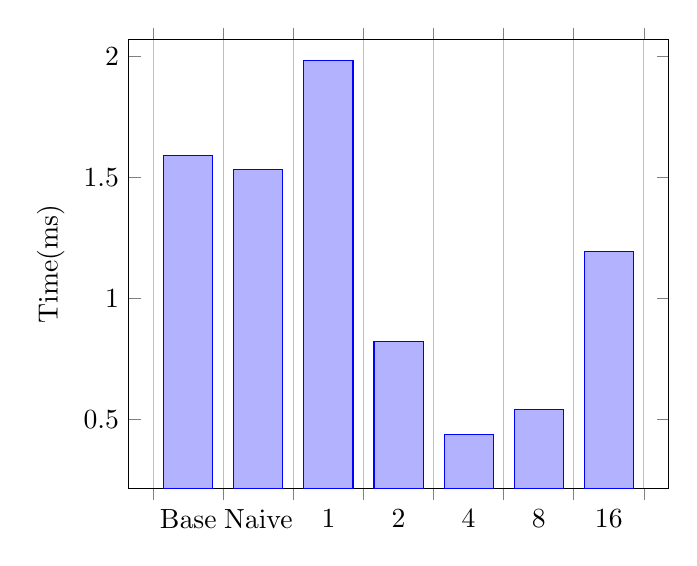
\begin{tikzpicture}
        \begin{axis}[
            ylabel=Time(ms),
            enlargelimits=0.05,
            legend style={at={(0.5,-0.1)},
            anchor=north,legend columns=-1},
            ybar interval=0.7,
            bar width=10pt,
            symbolic x coords={Base, Naive, 1,2,4,8,16, 17},
            xtick=data,
            ymin=.3
        ]
        \addplot % padded COO data
        coordinates {(Base, 1.59) (Naive, 1.534)(1,1.986) (2,0.822)
            (4,0.438) (8,0.542) (16, 1.196) (17, 1.196)};
        \end{axis}
    \end{tikzpicture}
    \caption{Evaluation over padding sizes, Batch size = 1e4, Lmax = 5}
    \label{fig:eval1}
\end{figure}
\subsection{Finetuning group size}
\label{sec:eval:group}
As seen in \autoref{fig:eval1} the group size parameter has a huge impact on the performance of the padded COO implementation. We've found
that performance across batch sizes for a certain group size was independent, but as lmax changed, the optimal group size would change as well.
This observation makes sense intuitively as changing lmax changes the number and distribution of non-zero entries in \textbf{W}, so a group size setting 
for a high lmax might add too many padding zeroes to compute compared to the contention it reduces in the tensor product. However, for all relevant lmax settings(1-5) had group size $\in [3, 5]$.
\begin{figure}
    \centering
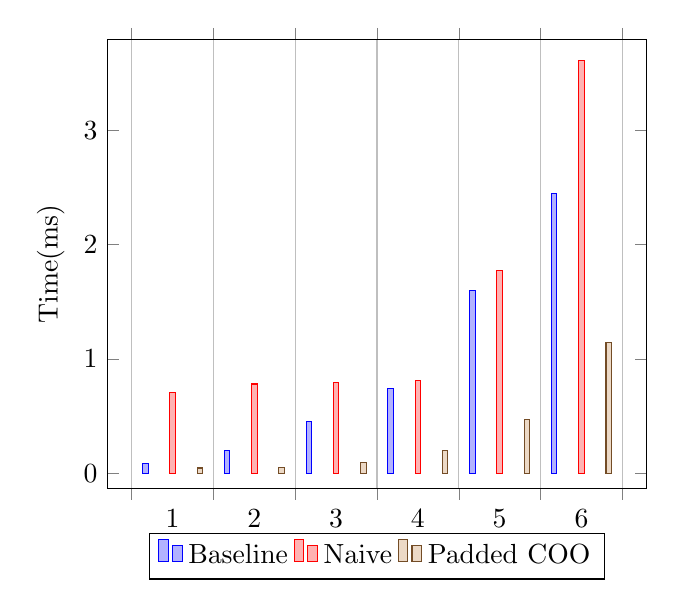
\begin{tikzpicture}
    \begin{axis}[
        x tick label style={
		/pgf/number format/1000 sep=},
        ylabel=Time(ms),
        enlargelimits=0.05,
        legend style={at={(0.5,-0.1)},
        anchor=north,legend columns=-1},
        ybar interval=0.2,
        bar width=1pt,
        symbolic x coords={1,2,3,4,5,6,7},
        xtick=data,
        ymin=.05,
    ]
    \addplot % padded COO data
    coordinates {(1, 0.089) (2, 0.199) (3, 0.457) (4, 0.742) (5, 1.6) (6, 2.451)(7,1)};
    \addplot % padded COO data
    coordinates {(1, 0.711) (2, 0.782) (3, 0.792) (4, 0.815) (5, 1.773) (6, 3.614) (7,1)};
    \addplot % padded COO data
    coordinates {(1, 0.047) (2, 0.05) (3, 0.096) (4, 0.201) (5, 0.472) (6, 1.148) (7,1)};
    \legend{Baseline, Naive, Padded COO}
    \end{axis}
\end{tikzpicture}
\label{fig:eval2}
\caption{Evaluation over Lmax, (Batch size = 1e4, Padding = 4)}
\end{figure}
\subsection{Impact of Lmax on performance}
\label{sec:eval:lmax}
As seen in \autoref{fig:eval2} we can see that Padded COO performs a factor of 4 times better than the baseline and Naive COO for all relevant lmax settings (1-5),
but baseline starts to catch up as lmax grows, with only a 2.5x speedup at lmax = 6. While the sparsity of the tensor product grows as lmax grows and therefore
the theorectical advantage of an implementation leveraged for that sparsity, it seems there are other factors at play limiting that advantage for this 
tensor product.

Combining that observation with the earlier observation that the group size does not change much with different lmax settings, we theorized
that while the sparsity increases with lmax, the distribution of non-zeroes migth be becoming adversarial to our padding approach. With some rudimentary analysis,
we saw that the distribution of non-zeroes per $k$ coordinate was skewed to the left but still maintained outliers at the max value, which increases with lmax.
Perhaps this skew is re-introducing the atomic add contention for some values of $k$ that were previously reduced by grouping, while also increasing the amount
of padding we need to add.

\begin{figure}
    \centering
    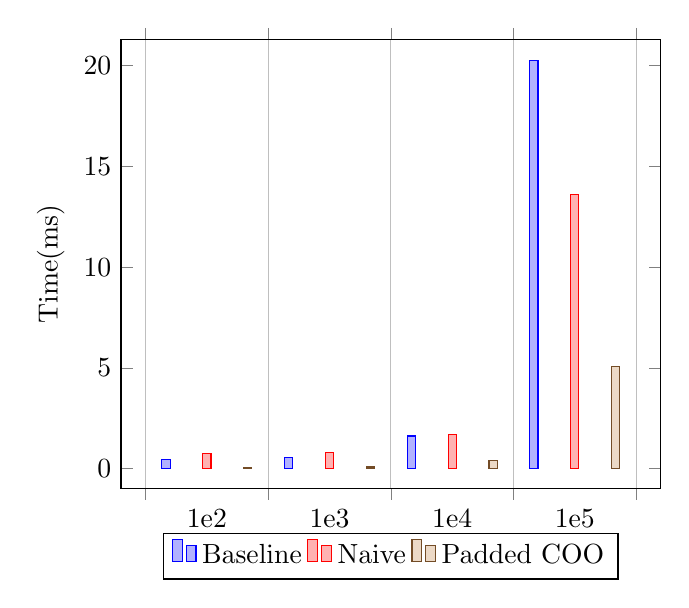
\begin{tikzpicture}
        \begin{axis}[
            x tick label style={
            /pgf/number format/1000 sep=},
            ylabel=Time(ms),
            enlargelimits=0.05,
            legend style={at={(0.5,-0.1)},
            anchor=north,legend columns=-1},
            ybar interval=0.2,
            bar width=1pt,
            symbolic x coords={1e2, 1e3, 1e4, 1e5, 7},
            xtick=data,
            ymin=.05
        ]
        \addplot % padded COO data
        coordinates {(1e2, 0.462) (1e3, 0.562) (1e4, 1.621) (1e5, 20.274) (7,1)};
        \addplot % padded COO data
        coordinates {(1e2, 0.762) (1e3, 0.782) (1e4, 1.711) (1e5, 13.628) (7,1)};
        \addplot % padded COO data
        coordinates {(1e2, 0.045) (1e3, 0.083) (1e4, 0.428) (1e5, 5.082) (7,1)};
        \legend{Baseline, Naive, Padded COO}
        \end{axis}
    \end{tikzpicture}
    \caption{Evaluation over Batch size, (Padding = 4, Lmax = 5)}
    \label{fig:eval3}   
\end{figure}
\subsection{Impact of batch size on performance}
As seen in \autoref{fig:eval3}, Padded COO performs at least a factor of 4 times better than the 
baseline and Naive COO for all batch sizes we could test, but had a bigger advantage at smaller batch sizes before 
speedup plateaued.
\section{Discussion} 
With our project, we successfully leveraged the structured sparsity within the \textbf{e3nn} tensor product to increase
the performance of the tensor product by 2-10x(4-10x for relevant parameters). We also showed that the performance of the
 padded COO implementation is independent of the batch size and group size settings. We also identified a potential scaling problem
 with our approach that would limit speedup on higher values of lmax. 
\subsection{Related Work}
For the tensor product itself, to the best of our knowledge the \textbf{e3nn-jax} tensor product is the state-of-the-art implementation, and 
there are no other public efforts to boost it's performance using it's intrinsic sparsity. While we ended up using Triton as our implementation 
of choice, we unsuccessfully attempted a lower level implementation using NVIDIA's cuSPARSE library\cite{nvidia_cusparse}; the many dimensions of the einsum and converting 
some of the necessary functions to prepare the benchmark from \textbf{e3nn} was too difficult compared to focusing our efforts on Triton.




    